% Autorska priprava k Realisticky.cz 020311, 020320; ulohy jsou autorske a obmenene.
% Zamerne nenahrazuje vyklad presnymi kopiemi cizich textu/prikladu.
\documentclass[11pt,a4paper]{article}
\input{../../sablony/pripravy/priprava.sty}
\usepackage{tikz}
\nastavPripravu{1. ročník}{Rovnice a nerovnice}{82}{Počet řešení soustavy a geometrie}
\begin{document}
\blok{Návaznost a motivace}
V hodinách lineárních funkcí jsme kreslili dvě přímky. Nyní stejnou geometrii využijeme ke klasifikaci soustav: protínající se, rovnoběžné a totožné přímky.
\begin{definiceBox}
\textbf{Geometrické řešení soustavy}. Společné body grafů rovnic soustavy. U dvou lineárních rovnic ve dvou neznámých může nastat jeden průsečík, žádný průsečík nebo nekonečně mnoho společných bodů.
\end{definiceBox}
\blok{Princip a odvození}
Rozhodující není jen zápis číslic, ale vzájemný vztah rovnic. Například $x+y=3$ a $2x+2y=6$ určují tutéž přímku; $x+y=3$ a $2x+2y=8$ dvě rovnoběžné přímky.

\begin{center}
\begin{minipage}[t]{.32\linewidth}\centering\small Jediný průsečík\\[-1mm]
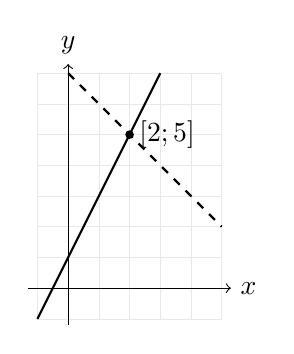
\begin{tikzpicture}[scale=.39]
\draw[step=1,gray!18,very thin] (-1,-1) grid (5,7);
\draw[->] (-1.3,0)--(5.3,0) node[right]{$x$};
\draw[->] (0,-1.2)--(0,7.3) node[above]{$y$};
\draw[thick] (-1,-1)--(3,7);
\draw[thick,dashed] (0,7)--(5,2);
\fill (2,5) circle (4pt) node[right]{$[2;5]$};
\end{tikzpicture}\end{minipage}\hfill
\begin{minipage}[t]{.32\linewidth}\centering\small Rovnoběžné\\[-1mm]
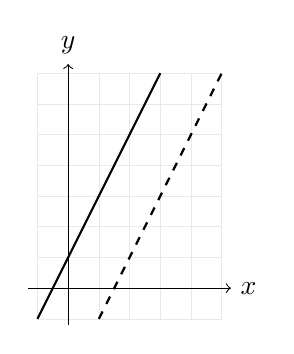
\begin{tikzpicture}[scale=.39]
\draw[step=1,gray!18,very thin] (-1,-1) grid (5,7);
\draw[->] (-1.3,0)--(5.3,0) node[right]{$x$};
\draw[->] (0,-1.2)--(0,7.3) node[above]{$y$};
\draw[thick] (-1,-1)--(3,7);
\draw[thick,dashed] (1,-1)--(5,7);
\end{tikzpicture}\end{minipage}\hfill
\begin{minipage}[t]{.32\linewidth}\centering\small Totožné\\[-1mm]
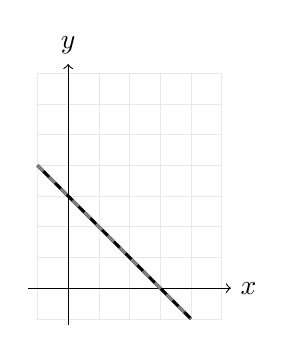
\begin{tikzpicture}[scale=.39]
\draw[step=1,gray!18,very thin] (-1,-1) grid (5,7);
\draw[->] (-1.3,0)--(5.3,0) node[right]{$x$};
\draw[->] (0,-1.2)--(0,7.3) node[above]{$y$};
\draw[very thick] (-1,4)--(4,-1);
\draw[very thick,dashed,gray] (-1,4)--(4,-1);
\end{tikzpicture}\end{minipage}
\end{center}
\blok{Řešené příklady: od jednoduchého ke složitějšímu}
\begin{prikladReseniBox}[title={Příklad 1}]
Určete počet řešení $\begin{cases}y=2x+1,\\y=-x+7.\end{cases}$
\tcblower
\[
\begin{aligned}
2x+1&=-x+7 \\
 3x&=6 \\
 x&=2,\quad y=5
\end{aligned}
\]

Jediný společný bod je $[2;5]$.
\[
\begin{aligned}
K &= \{[2;5]\}
\end{aligned}
\]
\end{prikladReseniBox}
\begin{prikladReseniBox}[title={Příklad 2}]
Určete počet řešení $\begin{cases}y=2x+1,\\y=2x-3.\end{cases}$
\tcblower
\[
\begin{aligned}
2x+1&=2x-3 \\
 1&=-3
\end{aligned}
\]

Přímky mají stejnou směrnici a různé absolutní členy.
\[
\begin{aligned}
K &= \varnothing
\end{aligned}
\]
\end{prikladReseniBox}
\poznamka{Na náčrtu doplň tři malé dvojice přímek. Nevyžaduj formální determinanty.}
\blok{Samostatné procvičování}
\begin{zadaniReseniBox}[title={Úloha 1}]
$\begin{cases}x+y=3,\\2x+2y=6.\end{cases}$
\tcblower
\[
\begin{aligned}
2(x+y)&=6 \\
 0&=0 \\[2mm]
K &= \{[t;3-t]\mid t\in\mathbb R\}
\end{aligned}
\]
\end{zadaniReseniBox}
\begin{zadaniReseniBox}[title={Úloha 2}]
$\begin{cases}x+y=3,\\2x+2y=8.\end{cases}$
\tcblower
\[
\begin{aligned}
2(x+y)&=6\ne8 \\
 6&=8 \\[2mm]
K &= \varnothing
\end{aligned}
\]
\end{zadaniReseniBox}
\begin{zadaniReseniBox}[title={Úloha 3}]
$\begin{cases}x+y=7,\\x-y=1.\end{cases}$
\tcblower
\[
\begin{aligned}
2x&=8 \\
 x&=4,\quad y=3 \\[2mm]
K &= \{[4;3]\}
\end{aligned}
\]
\end{zadaniReseniBox}
\blok{Volitelná rezerva}
\begin{zadaniReseniBox}[title={Úloha 1}]
Porovnejte $2x+2y=10$ a $x+y=5$.
\tcblower
\[
\begin{aligned}
2(x+y)&=10 \\
 x+y&=5
\end{aligned}
\]

Rovnice jsou ekvivalentní: jde o celou přímku, nikoli o jediný bod.
\[
\begin{aligned}
K &= \{[t;5-t]\mid t\in\mathbb R\}
\end{aligned}
\]
\end{zadaniReseniBox}
\blok{Domácí úkol}
\begin{zadaniReseniBox}[title={Domácí příprava}]
\begin{enumerate}[label=\alph*)]
\item
$\begin{cases}y=-x+2,\\y=-x+5.\end{cases}$
\item
$\begin{cases}2x+4y=8,\\x+2y=4.\end{cases}$
\item
$\begin{cases}y=x-1,\\y=-2x+5.\end{cases}$
\item
$\begin{cases}y=2x-3,\\y=-x+6,\end{cases}$.
\item
$\begin{cases}3x-6y=12,\\x-2y=5,\end{cases}$.
\item
$\begin{cases}4x+2y=10,\\2x+y=5,\end{cases}$.
\end{enumerate}
\tcblower
\begin{enumerate}[label=\alph*)]
\item
\[
\begin{aligned}
-x+2&=-x+5 \\
 2&=5 \\[2mm]
K &= \varnothing
\end{aligned}
\]
\item
\[
\begin{aligned}
2(x+2y)&=8 \\
 0&=0 \\[2mm]
K &= \{[4-2t;t]\mid t\in\mathbb R\}
\end{aligned}
\]
\item
\[
\begin{aligned}
x-1&=-2x+5 \\
 x&=2,\quad y=1 \\[2mm]
K &= \{[2;1]\}
\end{aligned}
\]
\item
\[
\begin{aligned}
2x-3&=-x+6\\x&=3,\quad y=3 \\[2mm]
K &= \{[3;3]\}
\end{aligned}
\]
\item
\[
\begin{aligned}
3(x-2y)&=15\ne12 \\[2mm]
K &= \varnothing
\end{aligned}
\]
\item
\[
\begin{aligned}
2x+y&=5\\y&=t,\quad x=\frac{5-t}{2} \\[2mm]
K &= \left\{\left[\frac{5-t}{2};t\right]\mid t\in\mathbb R\right\}
\end{aligned}
\]
\end{enumerate}
\end{zadaniReseniBox}
\poznamka{Orientační časové rozvržení: 5 + 12 + 12 + 10 + 6 = 45 min. Přednost má pochopení jádra; rezerva není součástí časového součtu. Domácí úlohy jsou určeny na samostatnou práci, řešení zůstávají učiteli.}
\end{document}
